\section{Ejercicio 2}
\hypersetup{hidelinks}
\begin{tcolorbox}[title=Listar solo 10 propiedades del recurso Jorge Luis Borges \href{http://www.wikidata.org/entity/Q909}{\nolinkurl{http://www.wikidata.org/entity/Q909}}]

  \begin{lstlisting}[language=SPARQL, breaklines=true]
    PREFIX rdf: <http://www.w3.org/1999/02/22-rdf-syntax-ns#>
    PREFIX rdfs: <http://www.w3.org/2000/01/rdf-schema#>
    PREFIX owl: <http://www.w3.org/2002/07/owl#>
    PREFIX wd: <http://www.wikidata.org/entity/>
    
    SELECT ?property ?value
    WHERE {
      wd:Q909 ?property ?value.
      ?property rdf:type owl:ObjectProperty.
    }
    LIMIT 10
  \end{lstlisting}
  \end{tcolorbox}


\begin{tcolorbox}[title=Listar lugar de nacimiento y muerte. La consulta debe retornar también los rdfs:label filtrados por lenguaje inglés (usar FILTER)]

  \begin{lstlisting}[language=SPARQL, breaklines=true]
    PREFIX wdt: <http://www.wikidata.org/prop/direct/>
    PREFIX rdf: <http://www.w3.org/1999/02/22-rdf-syntax-ns#>
    PREFIX rdfs: <http://www.w3.org/2000/01/rdf-schema#>
    PREFIX owl: <http://www.w3.org/2002/07/owl#>
    PREFIX wd: <http://www.wikidata.org/entity/>

    SELECT *
    WHERE {
      wd:Q909 wdt:P19 ?bornPlace.  # Obtiene la propiedad "place of birth" de Q909
      wd:Q909 wdt:P20 ?deathPlace.  # Obtiene la propiedad "place of death" de Q909
      ?bornPlace rdfs:label ?bornPlaceLabel.  # Obtiene los labels de los valores
      ?deathPlace rdfs:label ?deathPlaceLabel.  # Obtiene el label del lugar de muerte
      FILTER(LANG(?bornPlaceLabel) = "en").
      FILTER(LANG(?deathPlaceLabel) = "en").
    }


  \end{lstlisting}
  \end{tcolorbox}

  \begin{tcolorbox}[title=Usando CONSTRUCT\, crear un nuevo grafo con todos los premios recibidos por Borges (award received). Recuperando también los rdfs:label de esos premios y filtrarlos por idioma inglés (en).]

    \begin{lstlisting}[language=SPARQL, breaklines=true]
      PREFIX wdt: <http://www.wikidata.org/prop/direct/>
      PREFIX rdf: <http://www.w3.org/1999/02/22-rdf-syntax-ns#>
      PREFIX rdfs: <http://www.w3.org/2000/01/rdf-schema#>
      PREFIX owl: <http://www.w3.org/2002/07/owl#>
      PREFIX wd: <http://www.wikidata.org/entity/>

      CONSTRUCT {
        wd:Q909 wdt:P166 ?award.
        ?award rdfs:label ?awardLabel.
      }
      WHERE {
        wd:Q909 wdt:P166 ?award. # Obtiene awards de q909
        ?award rdfs:label ?awardLabel. # Obteniene los labels de los awards
        FILTER(LANG(?awardLabel) = "en").
      }
  
  
    \end{lstlisting}
    \end{tcolorbox}

    \begin{figure}[!h]
      \centering
      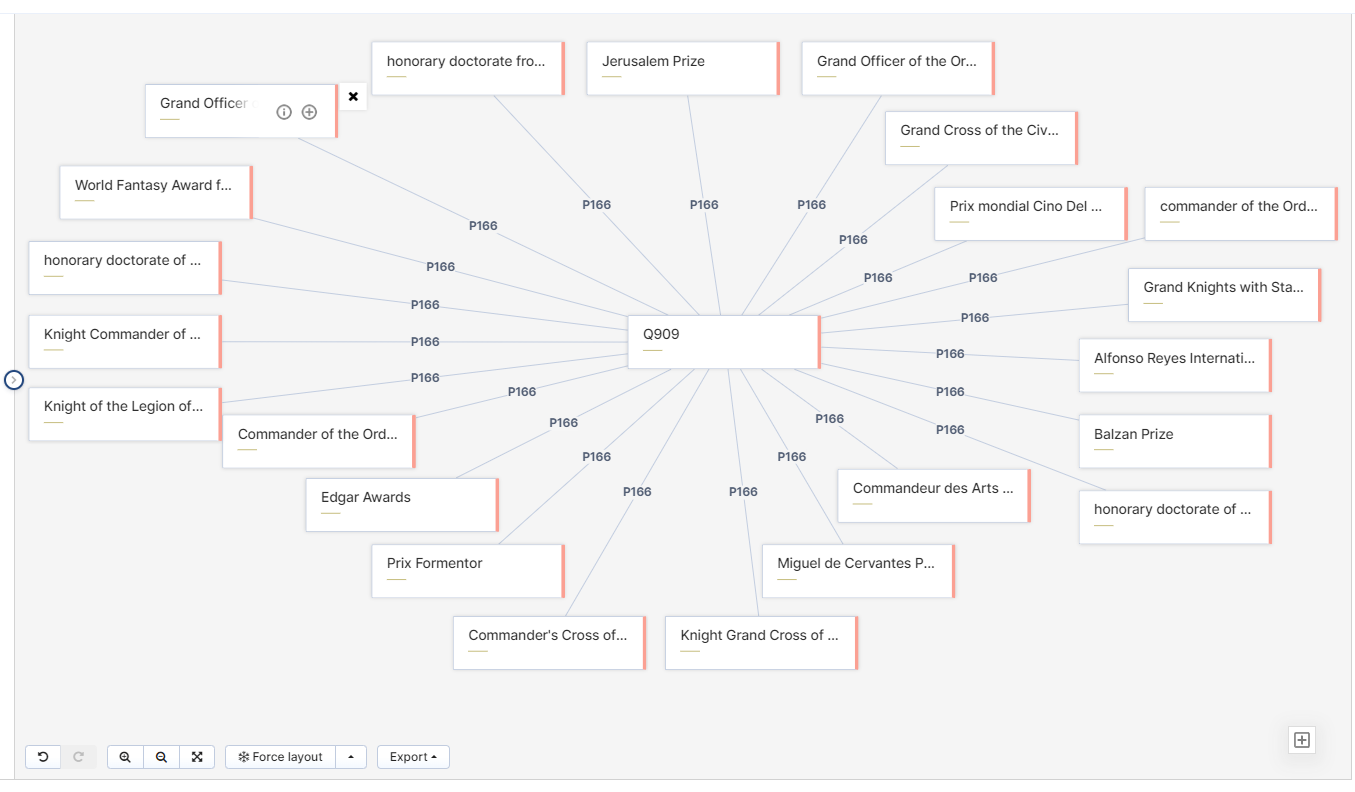
\includegraphics[width=16cm, scale=1]{Images/Imagenes/Grafo.png}
      \caption{Grafo de ``Awards'' de Borges obtenido con la ultima consulta SPARQL}
      \label{fig:marcado}
    \end{figure}